\documentclass{article}
\usepackage{caption}
\usepackage{mathtools}
\usepackage[UKenglish]{babel}
\usepackage[UKenglish]{isodate}
\usepackage{fullpage}
\usepackage{graphicx}
\usepackage{hyperref}
\usepackage{listings}
\usepackage{subcaption}
\usepackage{tikz-uml}
\usepackage[binary-units = true]{siunitx}

\title{Automated Benchmarking of Container Applications}
\author{Paulius Dilkas}

\begin{document}
\maketitle

%\begin{abstract}
%\end{abstract}

% TODO:
% Motivation
% OpenShift, MiniShift
% Prometheus
% Flink
% Docker

\section{Architecture and Implementation}

Two simple Dockerfiles were created. The first one is used for TaskManager and
JobManager pods and extends the original Flink Docker image by enabling
Prometheus support on port 9250. Prometheus can then query that port in order to
retrieve and record performance metrics.

The second Dockerfile extends the first one by adding a JAR file with Java code
for both the control server and the Flink app. This image also contains a custom
\texttt{ENTRYPOINT} that sends the Flink app to the JobManager (via port 8081)
as a background process, while executing the control server in the foreground.
This is the optimal arrangement of the two processes since the control server
always waits for the Flink app to finish in order to take its running time into
account when requesting data from Prometheus.

In both cases, one needs to change the permissions and group ownership of the
\texttt{/opt/flink} directory (to \texttt{775} and \texttt{root}, respectively)
so that the containers can be successfully executed by any user belonging to the
group \texttt{root}. Both images were put on Docker Hub, as this was the
simplest way to make them available to MiniShift.

A Docker Compose file was written with three services: Control,
JobManager, and TaskManager, establishing open ports as pictured in
Figure~\ref{fig:uml}). This file was then converted to OpenShift manifestos
using Kompose\footnote{\url{http://kompose.io/}}. The generated manifestos,
relevant network connections, and other dependencies are displayed in
Figure~\ref{fig:uml}. The entire system can then be updated and deployed by
generating a new JAR file using Maven, building and uploading the two
Dockerfiles, and recreating all components of the OpenShift configuration, as
described by the manifestos.

Prometheus add-on for
MiniShift\footnote{\url{https://github.com/minishift/minishift-addons/tree/master/add-ons/prometheus}}
was modified to disable OAuth-based authentication by replacing
\texttt{-skip-auth-regex=\^{}/metrics} with \texttt{-skip-auth-regex=\^{}/}.
Furthermore, its configuration file was updated to set both scrape and
evaluation intervals to 1 second and the list of targets to JobManager and
TaskManager, both on port 9250.

Configuration Files component represents a ConfigMap created using the
\texttt{oc} command that contains two configuration files, \texttt{global.yaml}
and \texttt{components.yaml} (see Figures \ref{fig:global} and
\ref{fig:components} for examples). The former contains basic networking
information along with two parameters that control the experiment
(\texttt{experimentLength} and \texttt{messagesPerSecond}) and a list of
metrics. The two experiment-specific parameters together define the frequency
and number of messages that the \texttt{ControlServer} will send to the
\texttt{Benchmarker}. Each metric is described with three properties:
\texttt{name}, \texttt{filename}, and \texttt{query}. The last one corresponds
to the name of the property as defined by Prometheus, while the other two are
used for data storage and plotting. The \texttt{components.yaml} configuration
file, on the other hand describes a sequence of processing stages, each with its
own CPU usage time, memory usage, and output data size (i.e., the amount of data
passed to the next stage).

\begin{figure}
  \centering
\begin{lstlisting}[escapeinside={(*}{*)}]
controlHostname: control
controlPort: 9998
prometheusHostname: prometheus
messagesPerSecond: 1
experimentLength: 3 # in seconds
metrics:
  - name: Throughput
    filename: throughput
    query: flink_taskmanager_job_task_operator_componentThroughput
  - name: Heap Usage ((*\si{\mebi\byte}*))
    filename: heap
    query: flink_taskmanager_Status_JVM_Memory_Heap_Used
  - name: CPU Load
    filename: cpu
    query: flink_taskmanager_Status_JVM_CPU_Load
\end{lstlisting}
  \label{fig:global}
  \caption{Example global configuration file}
\end{figure}

\begin{figure}
  \centering
\begin{lstlisting}[escapeinside={(*}{*)}]
- cpuTime: 5000 # in (*\si{\milli\second}*)
  memoryUsage: 100 # in (*\si{\mebi\byte}*)
  outputSize: 1 # in (*\si{\kibi\byte}*)
- cpuTime: 5000
  memoryUsage: 200
  outputSize: 1
\end{lstlisting}
  \label{fig:components}
  \caption{Example configuration file that defines a list of components with
    their resource requirements}
\end{figure}

\begin{figure}
  \centering
  \begin{tikzpicture}
    % components: first column
    \umlbasiccomponent[x=-6, y=3, fill=cyan!20]{Prometheus}
    \begin{umlcomponent}[fill=cyan!20]{Configuration Files}
      \umlbasiccomponent[x=-6, y=-2, fill=red!20]{Global}
      \umlbasiccomponent[x=-6, y=-4, fill=red!20]{Components}
    \end{umlcomponent}

    % components: second column
    \umlbasiccomponent[x=0, y=1]{Control Service}
    \begin{umlcomponent}{Control Pod}
      \umlbasiccomponent[x=0, y=-2, fill=red!20]{Control Server}
      \umlbasiccomponent[x=0, y=-4, fill=red!20]{Benchmarker}
    \end{umlcomponent}
    \umlbasiccomponent[x=0, y=-7]{Control Persistent Volume Claim}
    \umlbasiccomponent[x=0, y=-10]{Control Persistent Volume}

    % components: third column
    \umlbasiccomponent[x=6, y=3]{JobManager Service}
    \umlbasiccomponent[x=6, y=-1]{JobManager Pod}
    \umlbasiccomponent[x=6, y=-4]{TaskManager Service}
    \umlbasiccomponent[x=6, y=-8]{TaskManager Pod}

    % connections in second column
    \umlVHVassemblyconnector{Control Persistent Volume Claim}{Control Persistent Volume}
    \umlVHVassemblyconnector{Control Pod}{Control Persistent Volume Claim}
    \umlprovidedinterface[interface=998, with port, distance=2.5]{Control Server}
    \umlrequiredinterface[interface=998, with port]{Benchmarker}
    \umlHVassemblyconnector{Control Service}{Control Server-west-interface}
    \umlHVassemblyconnector{Control Service}{Benchmarker-east-interface}

    % connections between first and second columns
    \umlHVHassemblyconnector[interface={\space}, arm1=-2.3]{Benchmarker}{Global}
    \umlVHVassemblyconnector[interface={\space}]{Control Server}{Global}
    \umlVHVassemblyconnector[interface={\space}, arm1=-0.7]{Benchmarker}{Components}

    % Prometheus connections
    \umlHVHassemblyconnector[interface=HTTPS, arm1=-2, with port]{Control Server}{Prometheus}
    \umlassemblyconnector[interface=9250, arm1=1, with port]{Prometheus}{JobManager Service}
    \umlHVHassemblyconnector[interface=9250, arm1=8, with port]{Prometheus}{TaskManager Service}

    % column 3 connections
    \umlVHVassemblyconnector[interface={6123{,} 6124{,} 8081{,} 9250}, with port]{JobManager Pod}{JobManager Service}
    \umlVHVassemblyconnector[interface={6121{,} 6122{,} 9250}, with port]{TaskManager Pod}{TaskManager Service}
  \end{tikzpicture}
  \label{fig:uml}
  \caption{UML component diagram of the system, as deployed on MiniShift. Yellow
  components are OpenShift manifestos, while red components represent files
  (either Java classes or YAML configuration files). Network connections are
  shown with ports and have port numbers (or application-layer protocol names)
  displayed.}
\end{figure}

\begin{figure}
  \centering
  \begin{tikzpicture}
    \begin{umlseqdiag}
      \umlobject[no ddots]{Benchmarker}
      \umlobject[no ddots]{ControlServer}
      \umlobject[no ddots]{Prometheus}
      \umldatabase[no ddots]{PersistentVolume}
      \begin{umlcall}[op={initialise stream}]{Benchmarker}{ControlServer}
        \begin{umlfragment}[type=loop, label={$\forall$ messages}, inner xsep=7]
          \begin{umlcall}[op={message}, type=return]{ControlServer}{Benchmarker}
          \end{umlcall}
        \end{umlfragment}
      \end{umlcall}
      \begin{umlcall}[op={runtime}, type=return]{Benchmarker}{ControlServer}
      \end{umlcall}
      \begin{umlfragment}[type=loop, label={$\forall$ metrics}, inner xsep=6]
        \begin{umlcall}[op={query}, return={metric}]{ControlServer}{Prometheus}
        \end{umlcall}
        \begin{umlcall}[op={metric}]{ControlServer}{PersistentVolume}
        \end{umlcall}
      \end{umlfragment}
    \end{umlseqdiag}
  \end{tikzpicture}
  \label{fig:communication}
  \caption{Communication between different parts of the system visualised as a
    UML sequence diagram}
\end{figure}

We illustrate some aspects of the execution and how different components
communicate with each other in Figure~\ref{fig:communication}. After the Flink
app (called Benchmarker) is initialised, it immediately establishes the control
server as a \texttt{socketTextStream}, i.e., the initial source of data. It then
constructs a chain of mappers according to the \texttt{components.yaml}
specifications.

The control server periodically sends messages to Benchmarker (as defined in
\texttt{global.yaml}). Each component (mapper) does three things upon receiving
each message:
\begin{enumerate}
\item First, it allocates an array so that the total memory usage would be as
  close to \texttt{memoryUsage} as possible. The array size is calculated using
  a linear regression model established using experimental data (see
  Section~\ref{sec:adjustments}).
\item Then, it creates a \texttt{String} object taking up \SI[number-math-rm =
  \mathnormal, parse-numbers = false]{\texttt{outputSize}}{\kibi\byte} of
  memory. This string will be passed to the next component in the chain.
\item Finally, it spends the remaining time (until total execution time is
  exactly \texttt{cpuTime}) testing the Collatz conjecture \cite{collatz} one
  initial integer at a time.
\end{enumerate}

After all messages from the control server pass through every mapper,
Benchmarker connects to the control server, sending it total running time (as
measured by \texttt{JobExecutionResult.getNetRuntime()}). This number is then
rounded up to an integer number of minutes and used to retrieve performance data
for the time interval when the application was running.

Finally, for each metric defined in the global configuration file, the control
server establishes an HTTPS connection to Prometheus, collects JSON data
recording the values of that metric in the last few minutes (as calculated
previously), and writes the data to a file (separate for each metric) on the
persistent volume.

The last component of the system consists of two Python scripts. The first is
responsible for deploying the entire OpenShift setup, waiting for the control
server to terminate, and using MiniShift SSH to copy files from the persistent
volume to a host folder, which places them into a local directory on the host
machine. The second script can then read the data and plot it using Matplotlib,
comparing observed data with their expected values, as dictated by the
parameters of the experiment.

\section{Local Performance Tuning} \label{sec:adjustments}

The component script, responsible for using predefined amounts of resources, was
tested and adjusted locally, ensuring that it uses 100\% of a single CPU and
\SI[number-math-rm = \mathnormal, parse-numbers =
false]{\texttt{memoryUsage}}{\mebi\byte} of memory. Total heap memory usage was
measured for array sizes $2^0, 2^1, 2^2, \dots, 2^9$ and output strings of $2^0,
2^1, 2^2, \dots, \min \{ 2^8, \text{array size} \}$ characters (the output
string is constructed using the array, so the array size must always be at least
as big as the output string). Maximum heap usage was measured using GNU
Time\footnote{\url{https://www.gnu.org/software/time/}} and its Maximum Resident
Set Size metric. Each experiment was repeated three times, and median values
were taken.

We seek to know the average amount of memory used by a single character of a
Java string. Knowing that a byte on an array takes up exactly one byte allows us
to reformulate the problem to a simple linear regression shown in
Figure~\ref{fig:regression1}. The model shows that overall memory usage can be
expressed as
\begin{equation} \label{eq:regression}
  \text{memory usage} = \SI{40}{\mebi\byte} + \text{array size} + 3.268 \times
  \text{string size} + \epsilon,
\end{equation}
contradicting the common wisdom that a character uses approximately two bytes of
memory \cite{java_memory}.

\begin{figure}
  \centering
  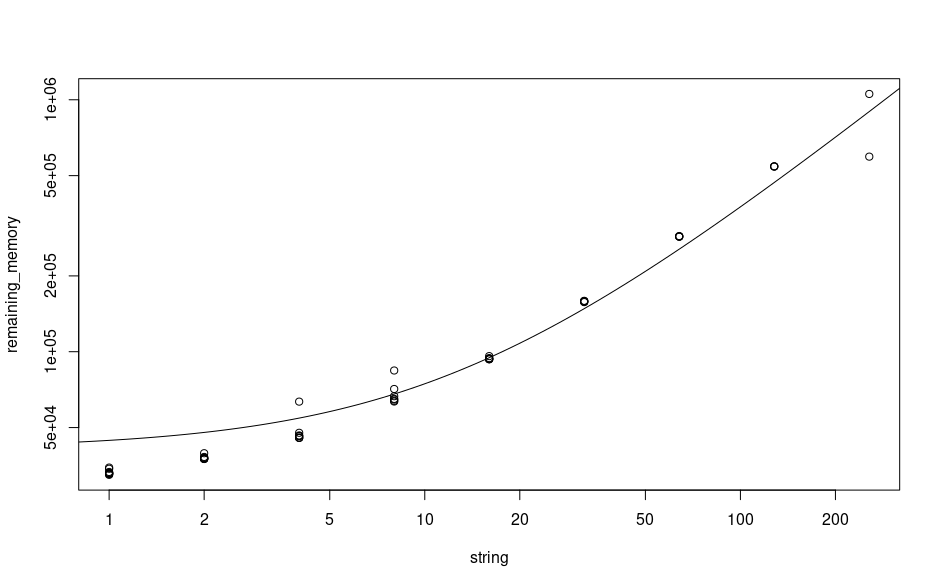
\includegraphics[width=\textwidth]{../proof_of_concept/prediction2.png}
  \caption{A log-log plot comparing the number of characters in a string and the
  observed memory unaccounted by the array. In each column, separate points
  correspond to different array sizes. The curve is a best-fit linear regression
  line.}
  \label{fig:regression1}
\end{figure}

Figure~\ref{fig:regression2} presents a more detailed view, however suggesting
the same conclusion. While the predictions seem to consistently overestimate
memory consumption for short strings and similarly underestimate it for longer
strings, adding a quadratic term is not enough to remove the bias in errors, and
the errors are sufficiently small (see Section~\ref{sec:after_adjustments} for
more details).

\begin{figure}
  \centering
  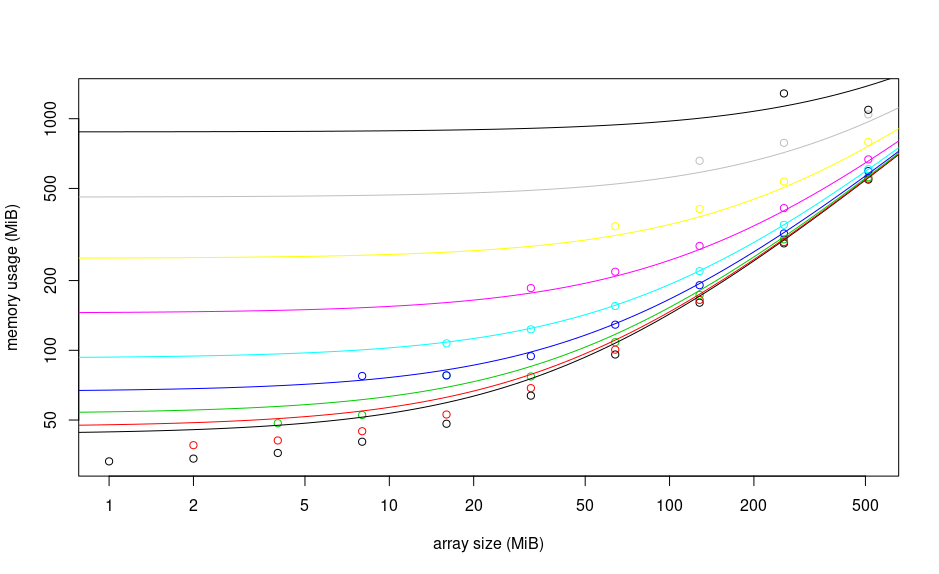
\includegraphics[width=\textwidth]{../proof_of_concept/prediction1.png}
  \caption{A log-log plot showing memory consumption across a range of array
    sizes, with different string sizes represented by different colours. For
    each string size, we also draw a regression line in the corresponding
    colour.}
  \label{fig:regression2}
\end{figure}

\subsection{Adjusted Performance} \label{sec:after_adjustments}

We can use the two numerical parameters in Equation~\eqref{eq:regression} to
adjust our `mapping function' in order to ensure that it uses the correct amount
of memory. We run a similar set of experiments as before, except replacing array
size with expected memory usage as one of our independent variables (the other
being string size). Memory usage is set to four different values: 64, 128,
256, and \SI{512}{\mebi\byte} (note that the smallest possible memory usage is
about \SI{40}{\mebi\byte}), while string size is exponentially increased from
\SI{1}{\mebi\byte} up to the largest power of two small enough so that the
string can be constructed from the array. We plot the errors in
Figure~\ref{fig:adjustment}. Note that the largest error is smaller than
\SI{50}{\kibi\byte}, which is good enough for our needs.

\begin{figure}
  \centering
  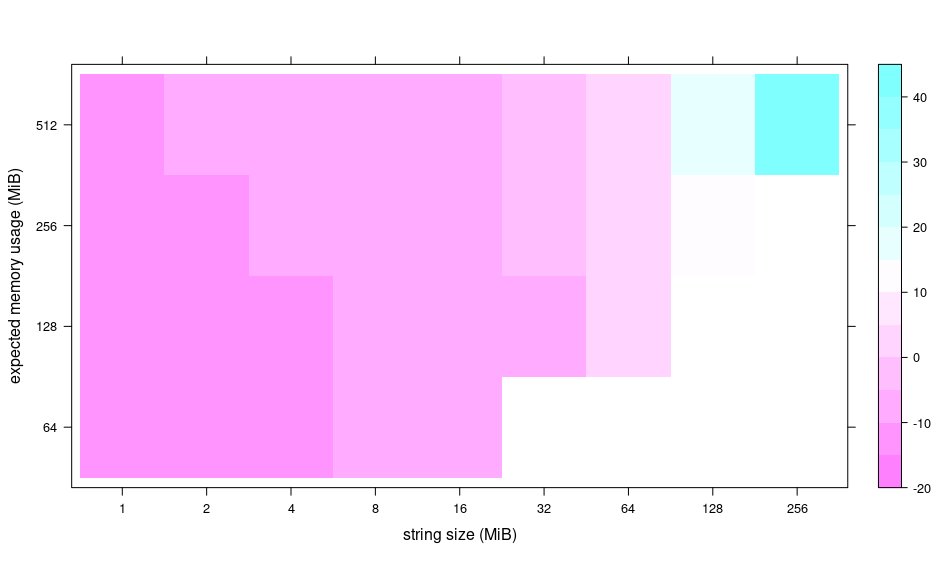
\includegraphics[width=\textwidth]{../proof_of_concept/adjusted.png}
  \caption{A heat map of errors (in \si{\kibi\byte})}
  \label{fig:adjustment}
\end{figure}

\section{Experimental Evaluation}
% TODO: a study that (visually) compares expected performance with Prometheus
% graphs for a range of (one-component) configurations

% TODO: explain the setup (according to experiment.py)
% measured at 1 s intervals

Experiments were performed in order to determine how well performance metrics
observed with a standalone Java application transfer to MiniShift. We explore
four values of \texttt{memoryUsage} (\SI{64}{\mebi\byte}, \SI{128}{\mebi\byte},
\SI{256}{\mebi\byte}, \SI{512}{\mebi\byte}), while keeping \texttt{cpuTime} at 0
so that each run lasts only as long as it takes to allocate and randomise the
memory. For \texttt{outputSize}, we explore every power-of-two number of
\si{\mebi\byte} compatible with the current \texttt{memoryUsage} value.

% TODO: and repetitions

\begin{figure}
  \centering
  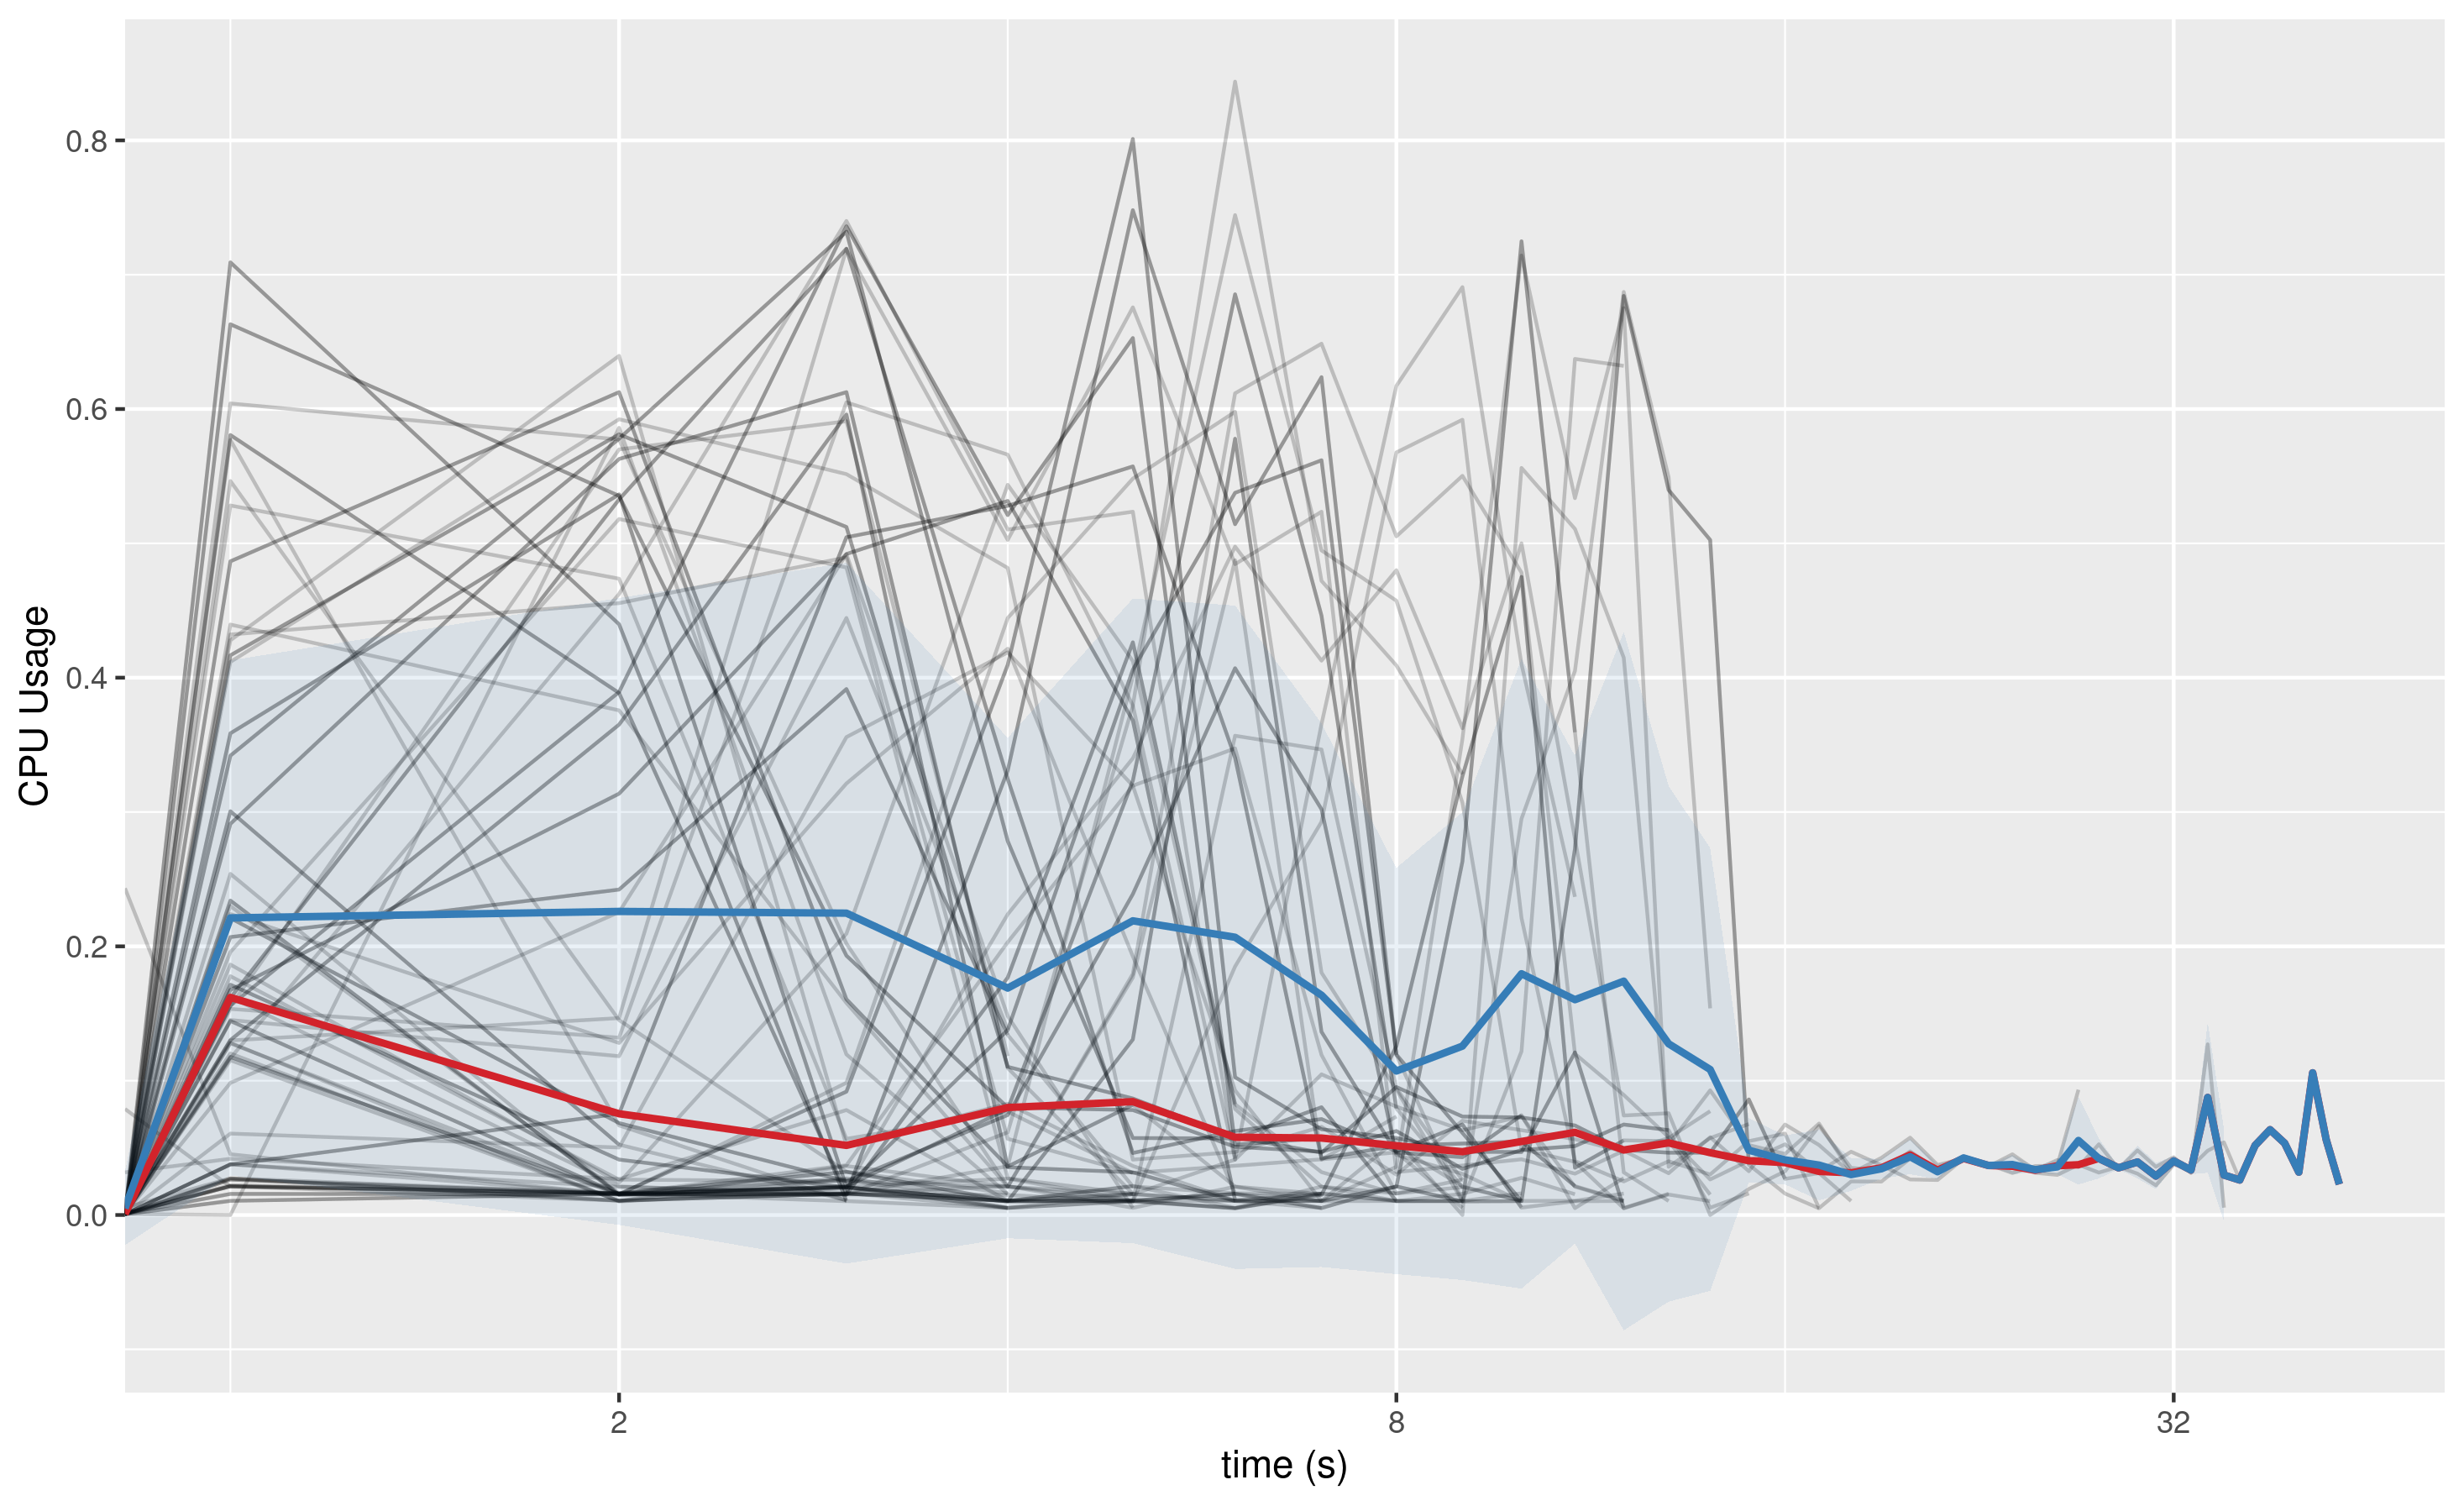
\includegraphics[width=\textwidth]{../plots/cpu_experiment.png}
  \caption{CPU usage across time. Each gray line represents a different run. The
  red curve is their (pointwise) median, the blue curve is the mean, while the
  shaded area marks 1 standard deviation around the mean. Note that time is on a
  $\log$ scale.}
  \label{fig:cpu_experiment}
\end{figure}

\begin{figure}
  \centering
  \begin{subfigure}[t]{0.49\textwidth}
    \centering
    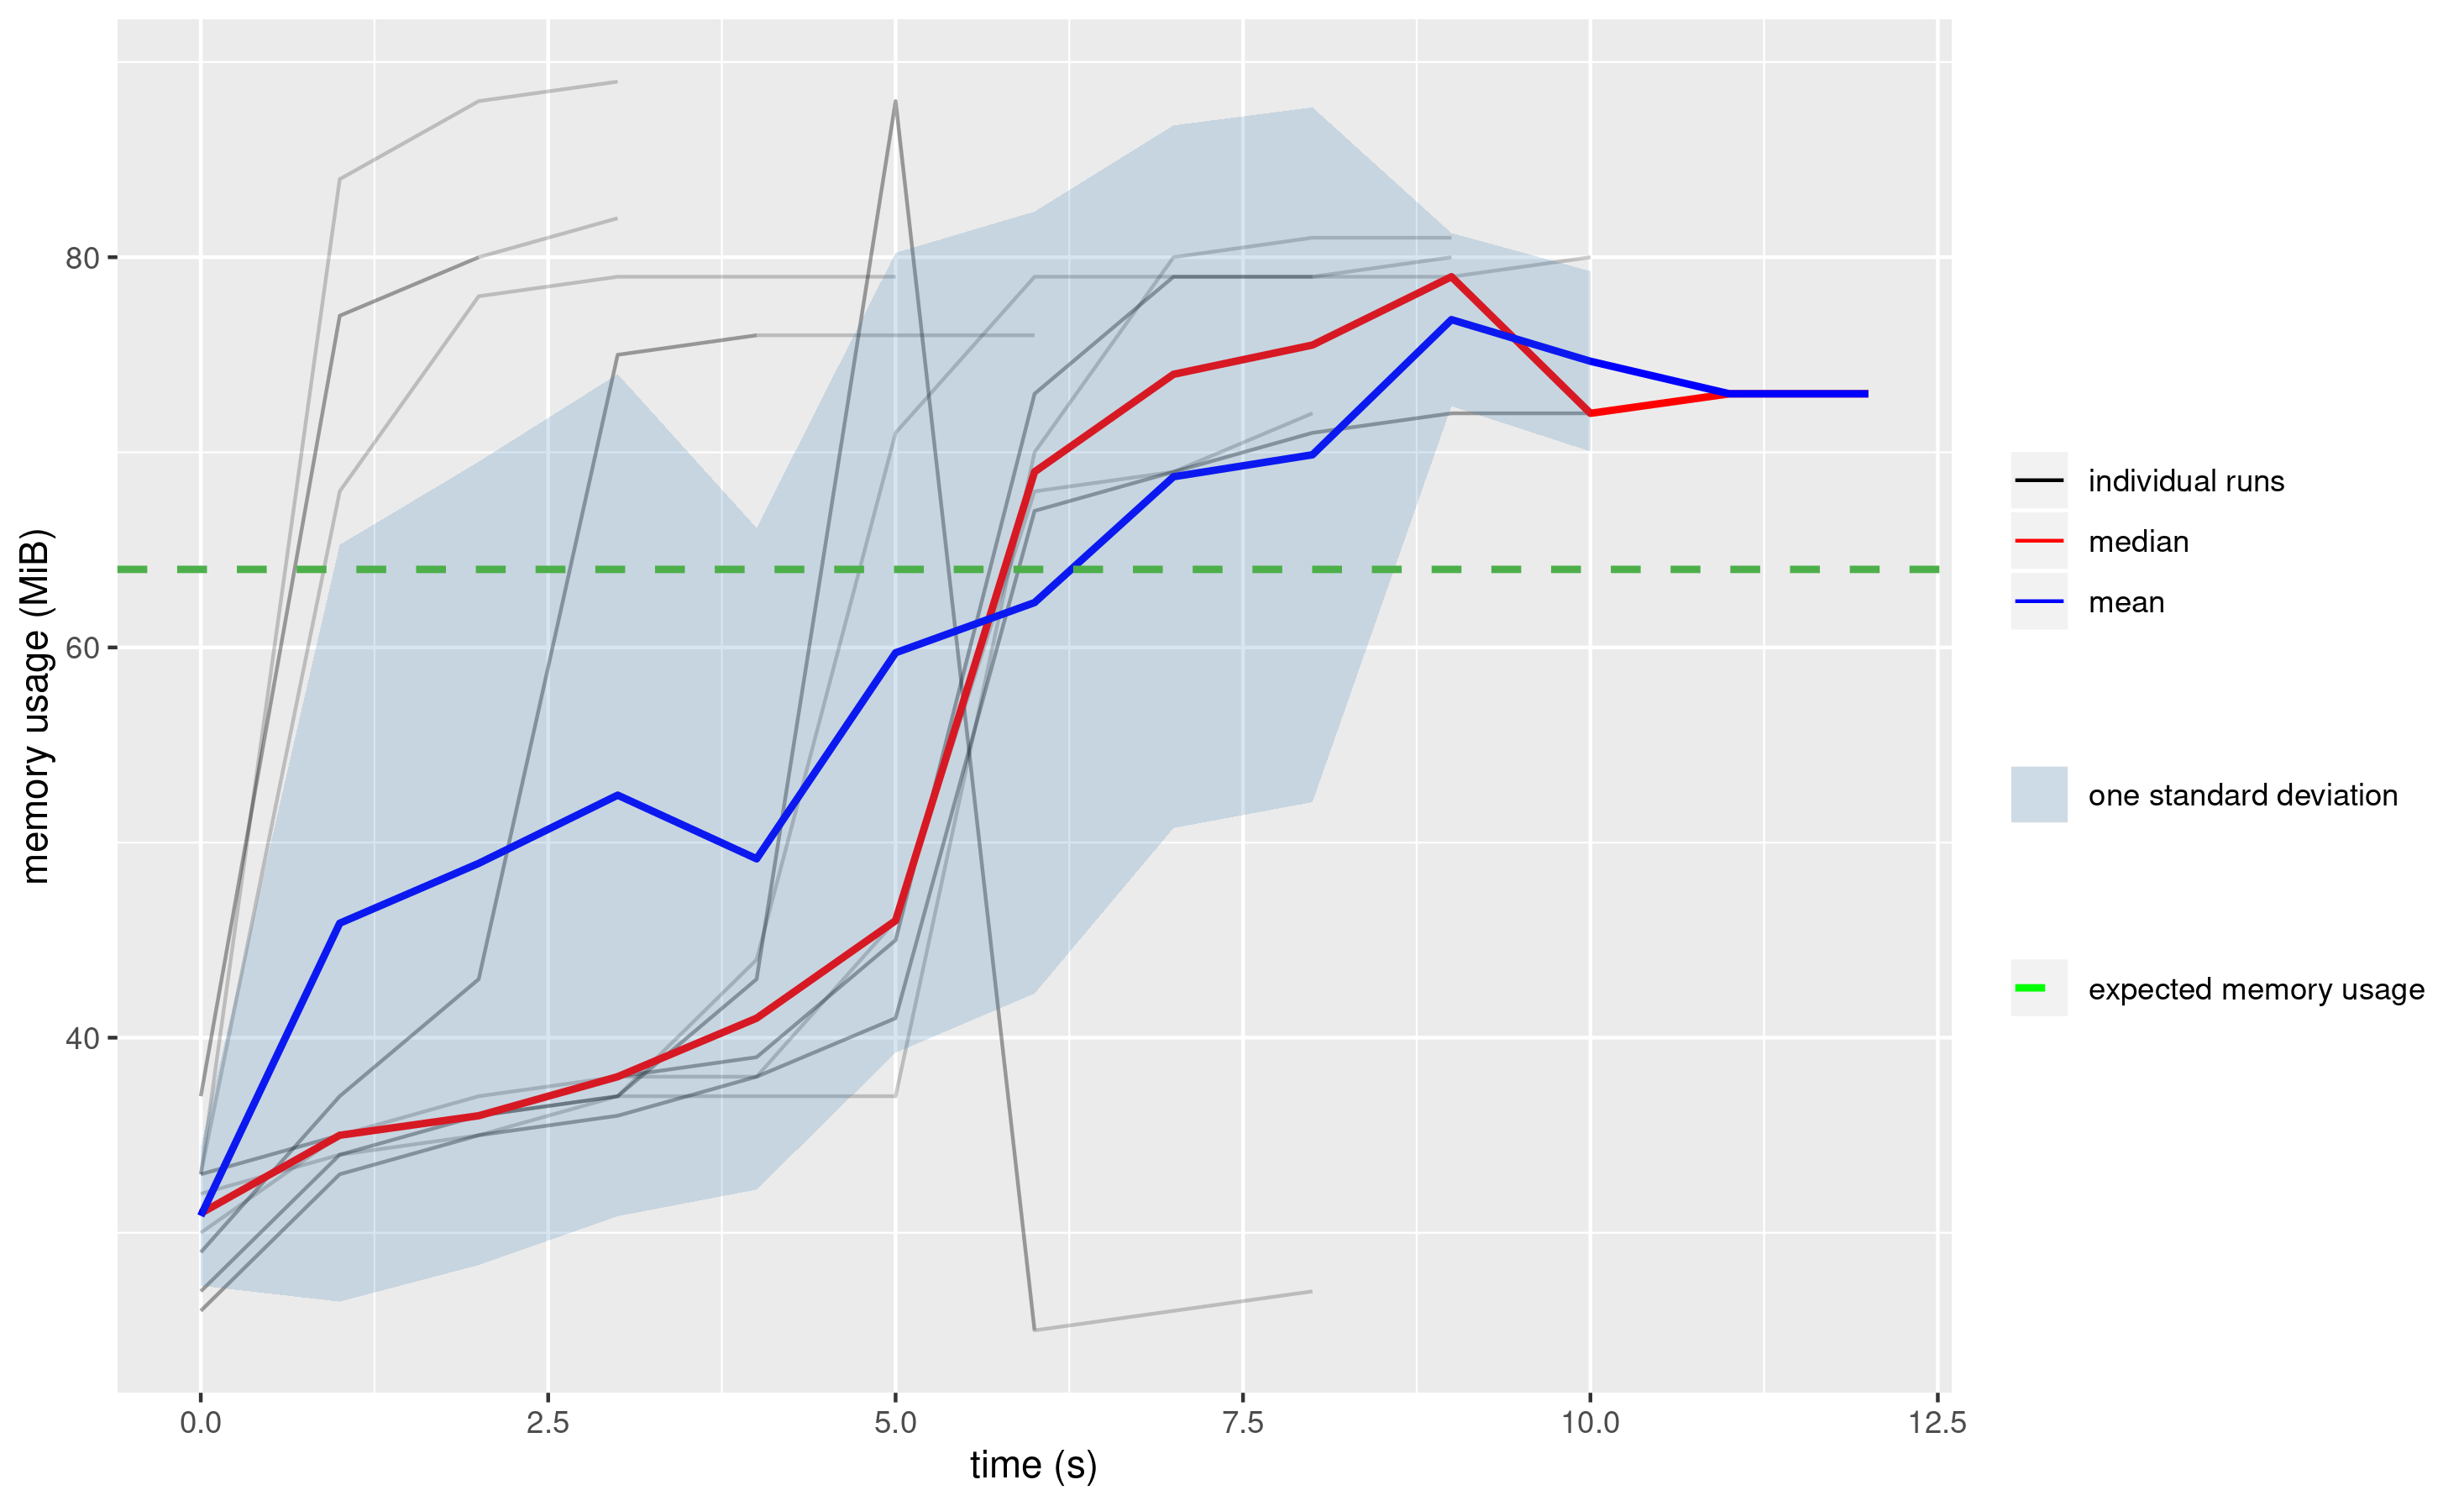
\includegraphics[width=\textwidth]{../plots/heap_64.png}
    \caption{expected heap usage: \SI{64}{\mebi\byte}}
    \label{fig:heap_64}
  \end{subfigure}
  \begin{subfigure}[t]{0.49\textwidth}
    \centering
    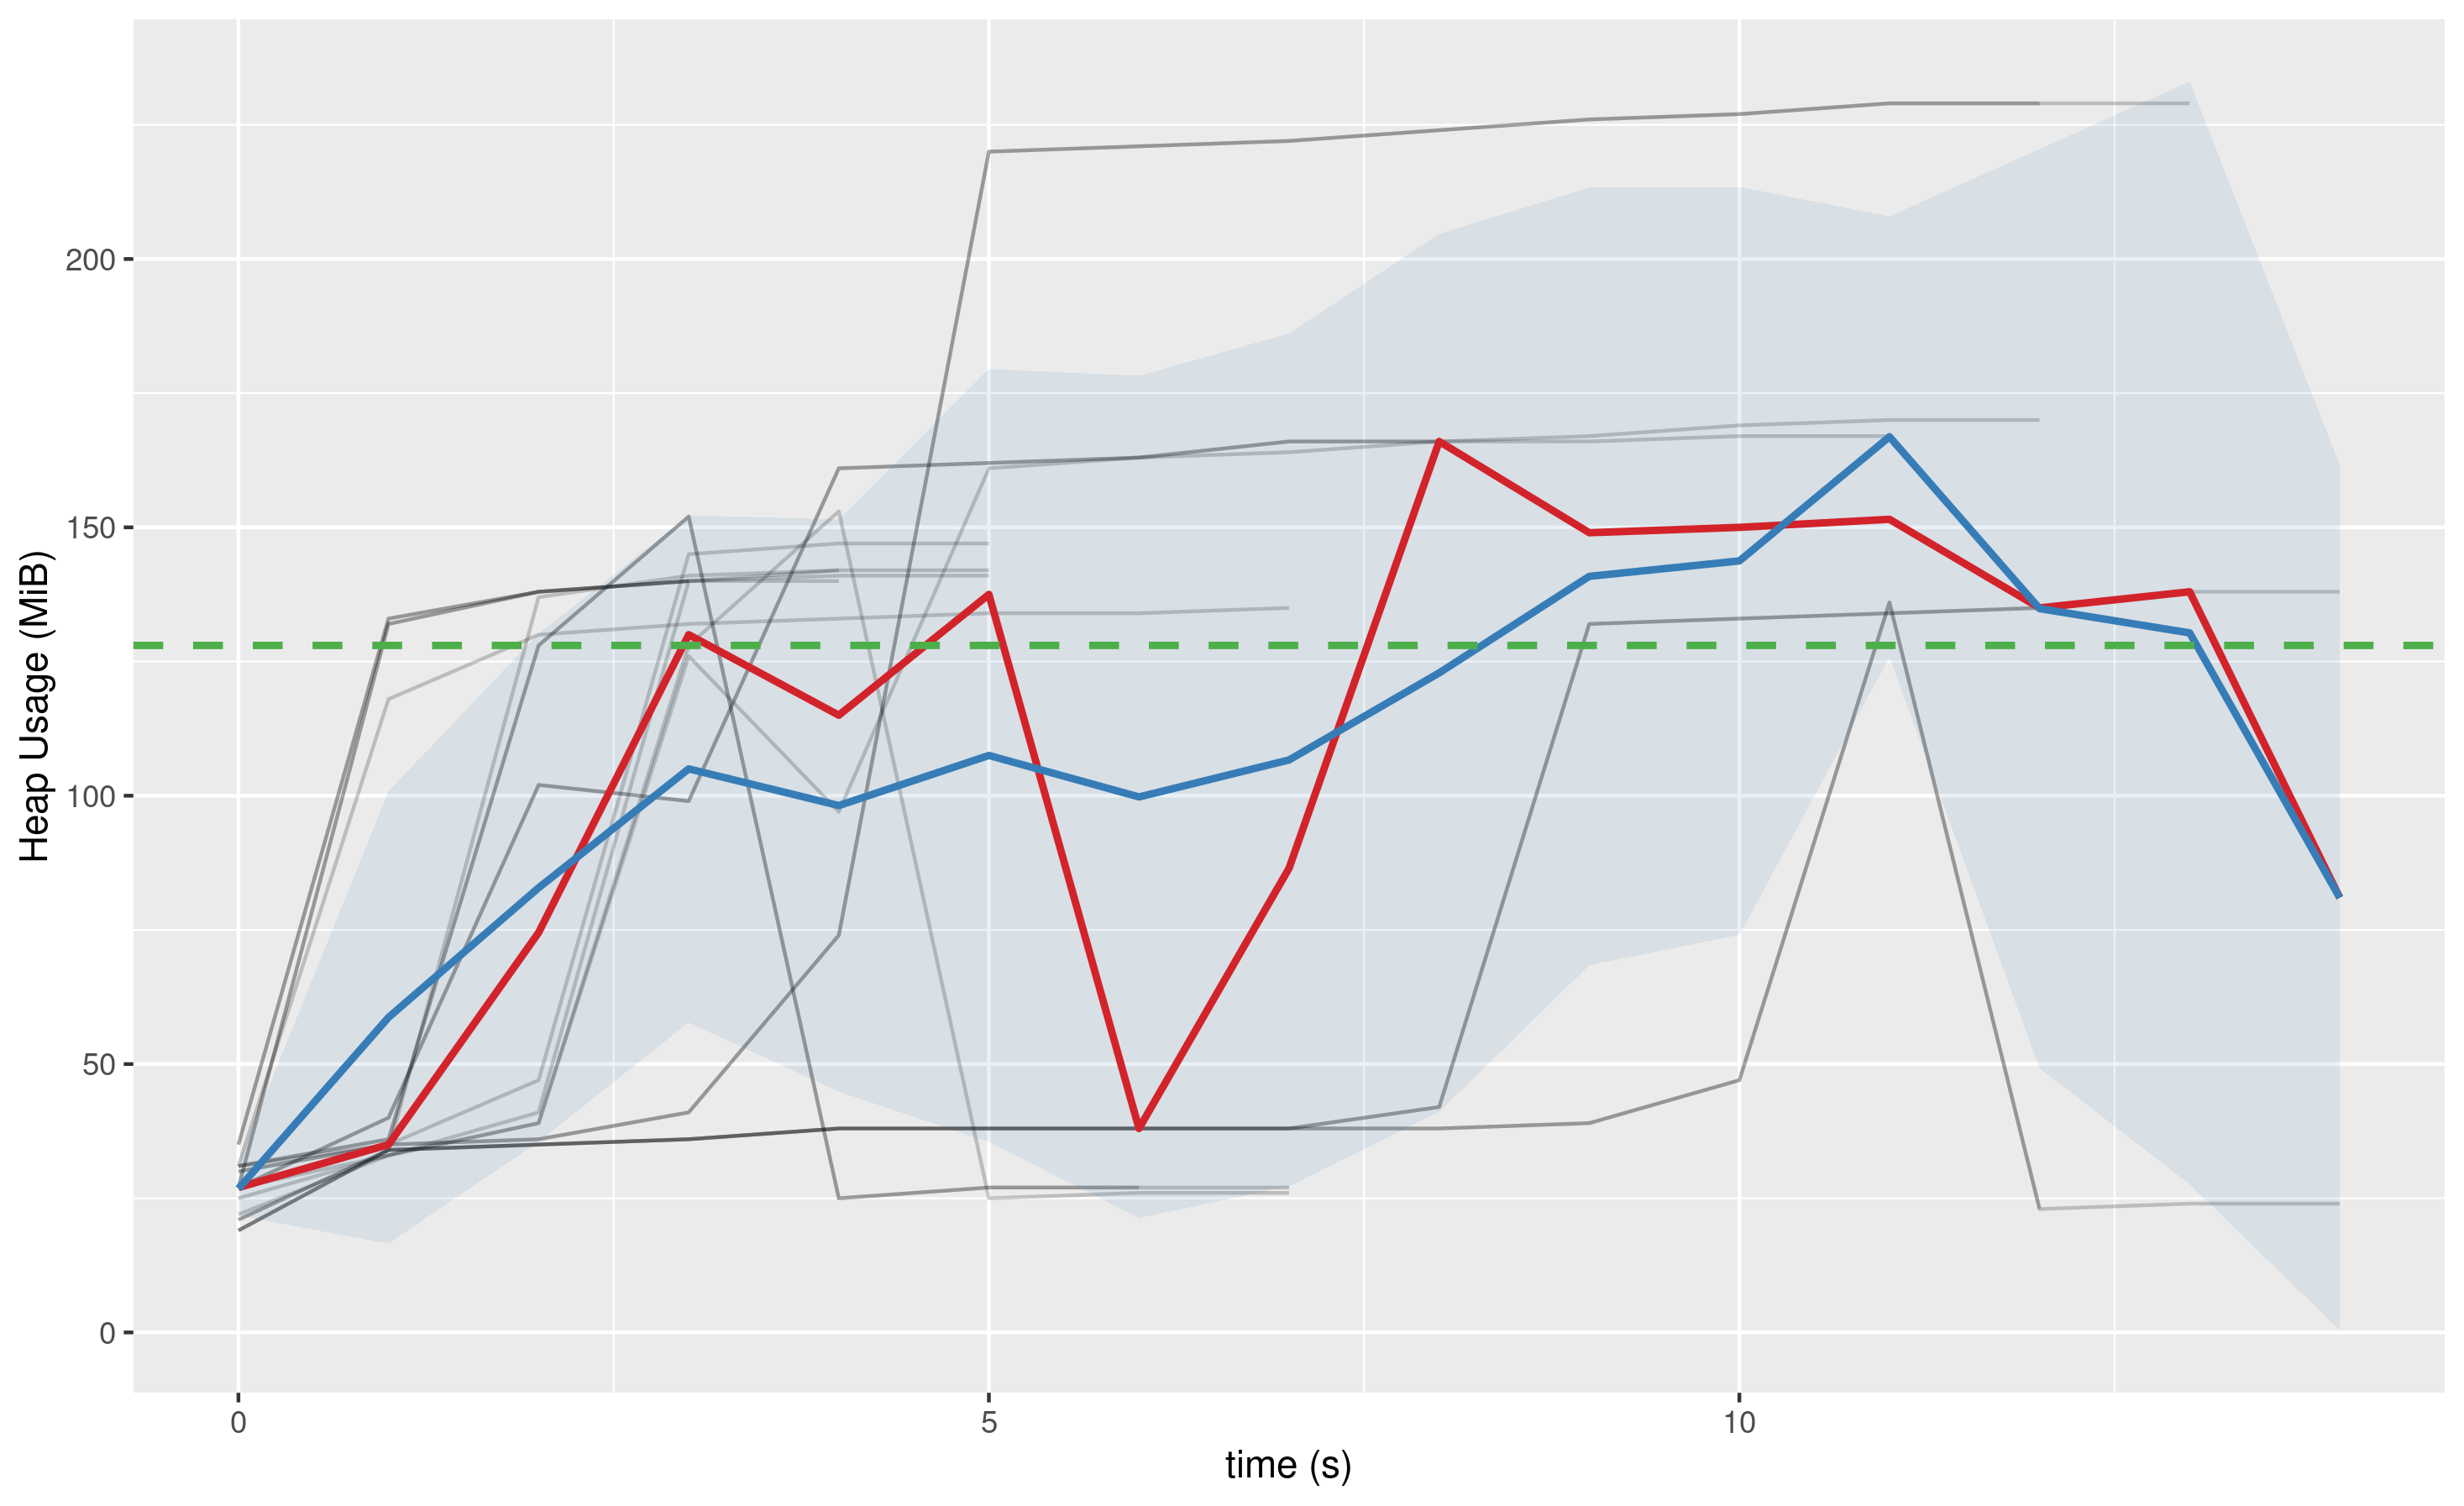
\includegraphics[width=\textwidth]{../plots/heap_128.png}
    \caption{expected heap usage: \SI{128}{\mebi\byte}}
    \label{fig:heap_128}
  \end{subfigure}
  \begin{subfigure}[t]{0.49\textwidth}
    \centering
    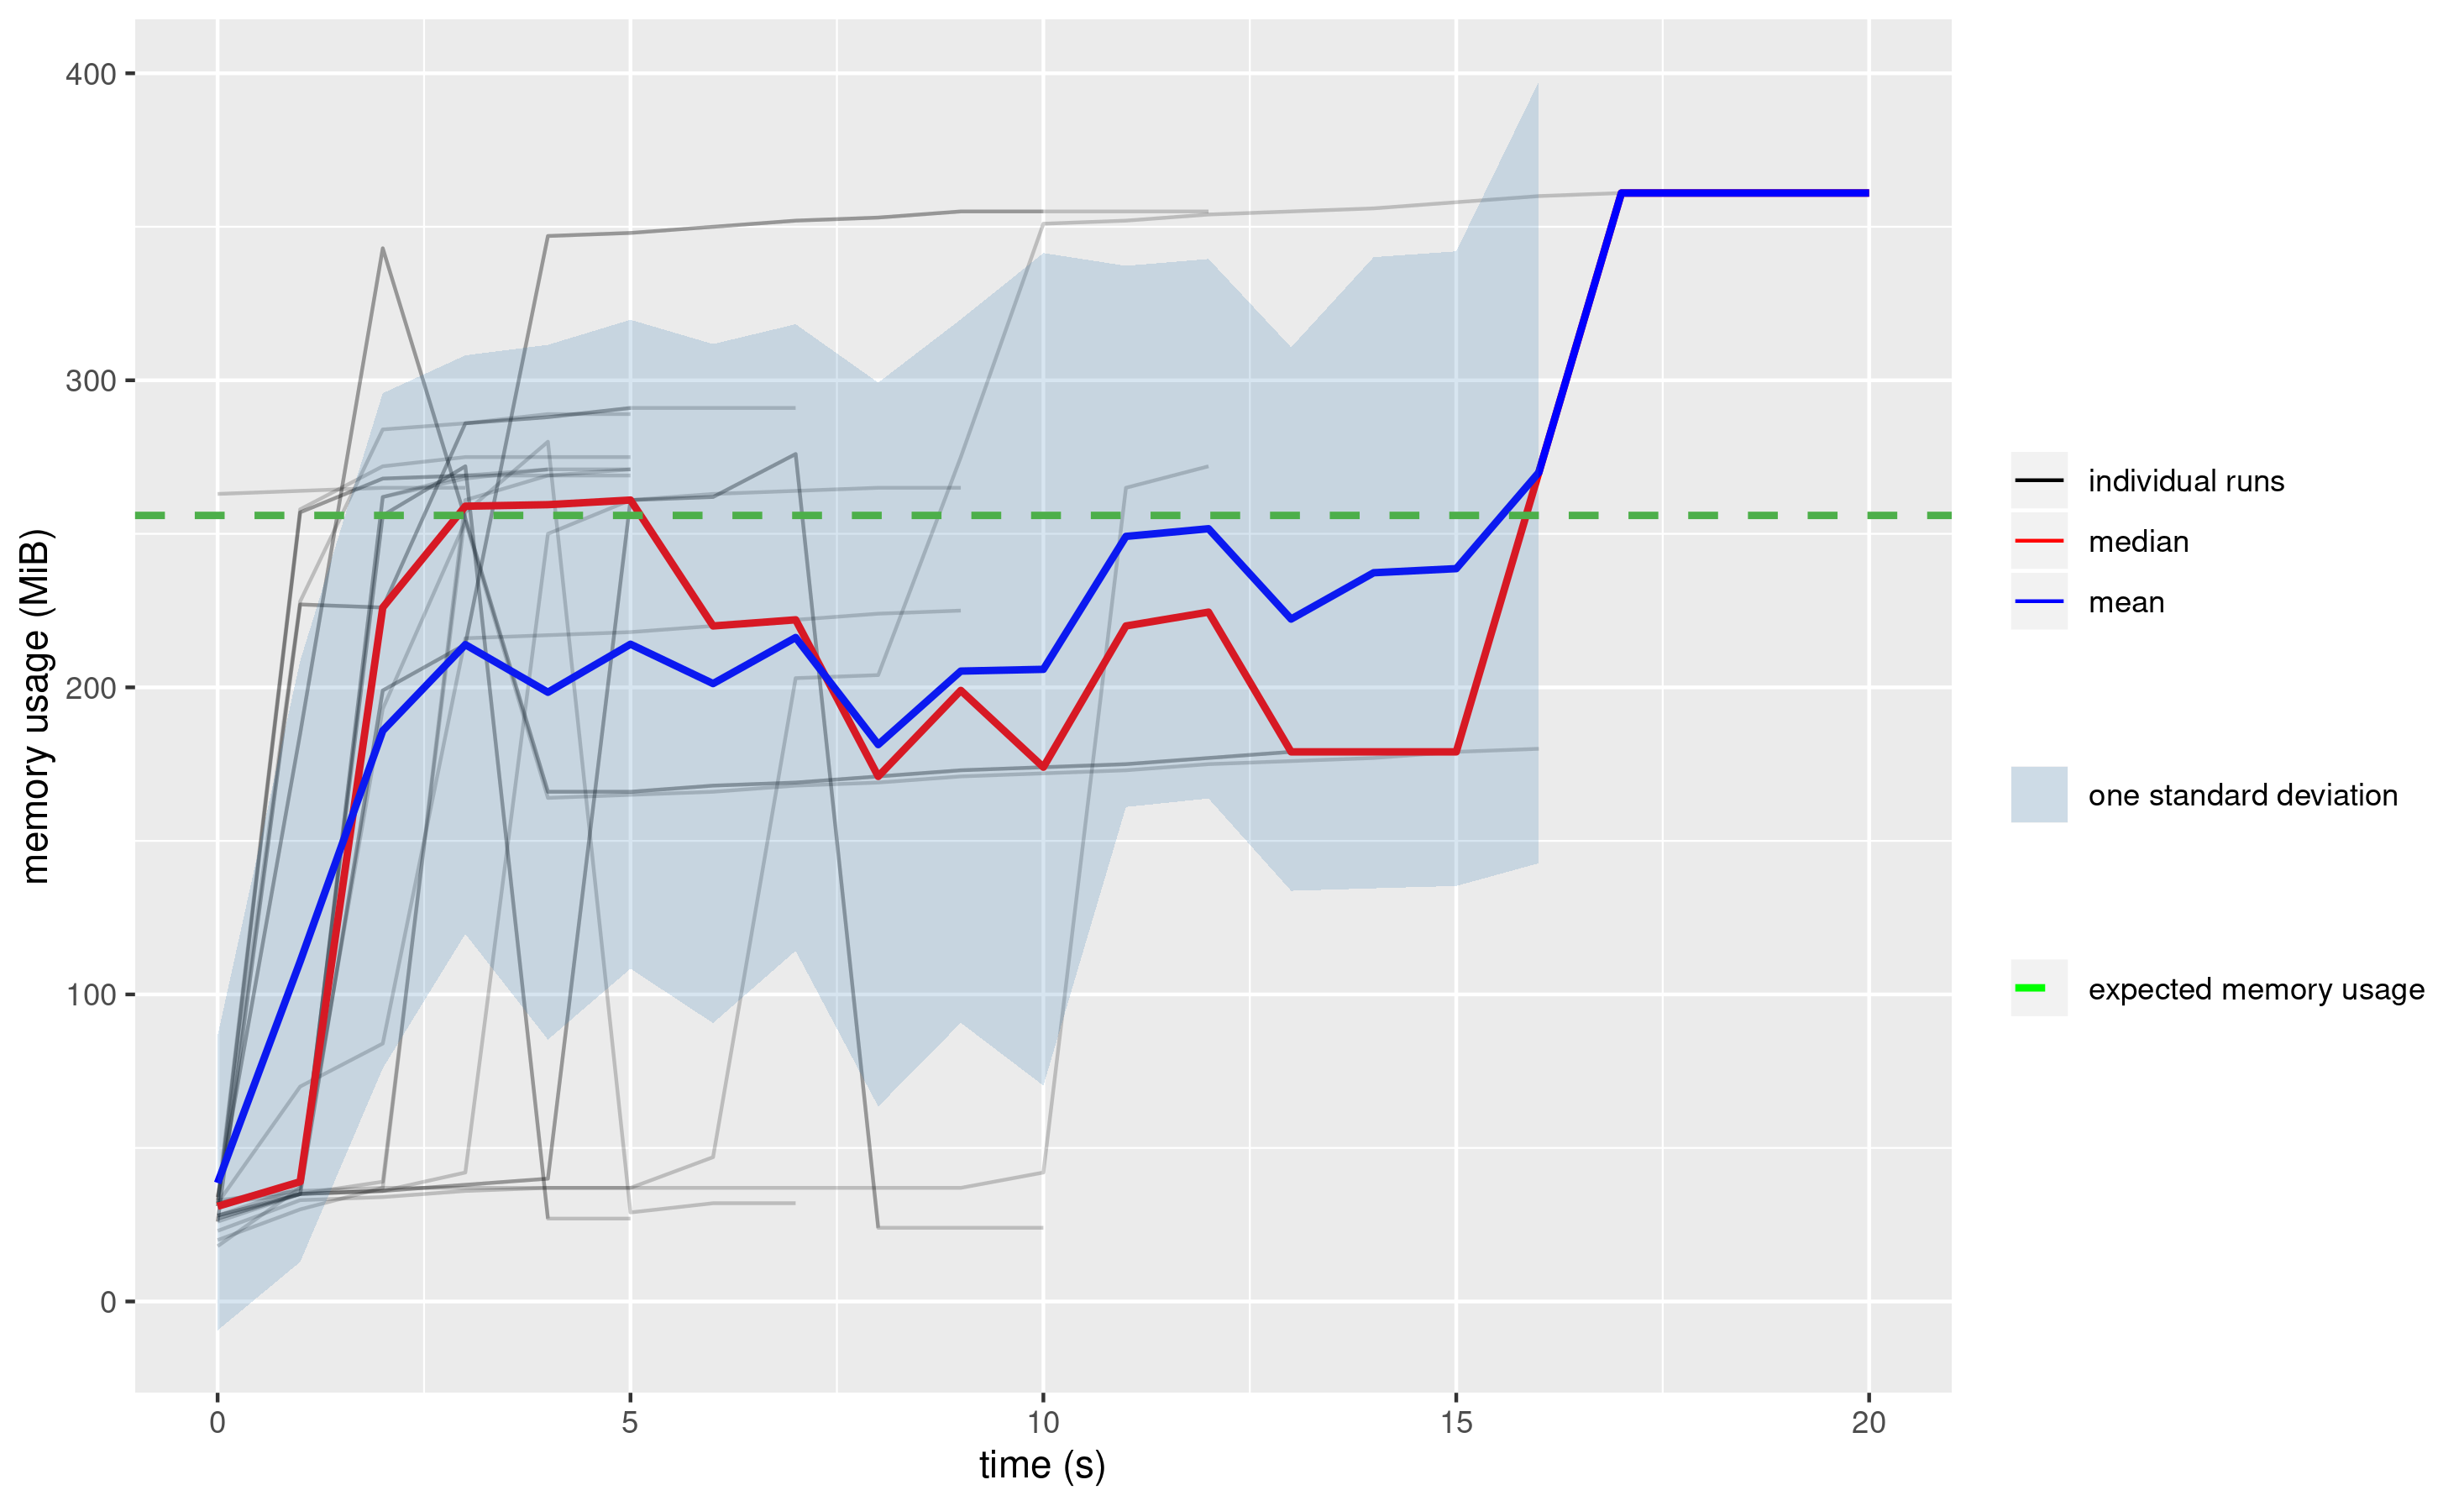
\includegraphics[width=\textwidth]{../plots/heap_256.png}
    \caption{expected heap usage: \SI{256}{\mebi\byte}}
    \label{fig:heap_256}
  \end{subfigure}
  \begin{subfigure}[t]{0.49\textwidth}
    \centering
    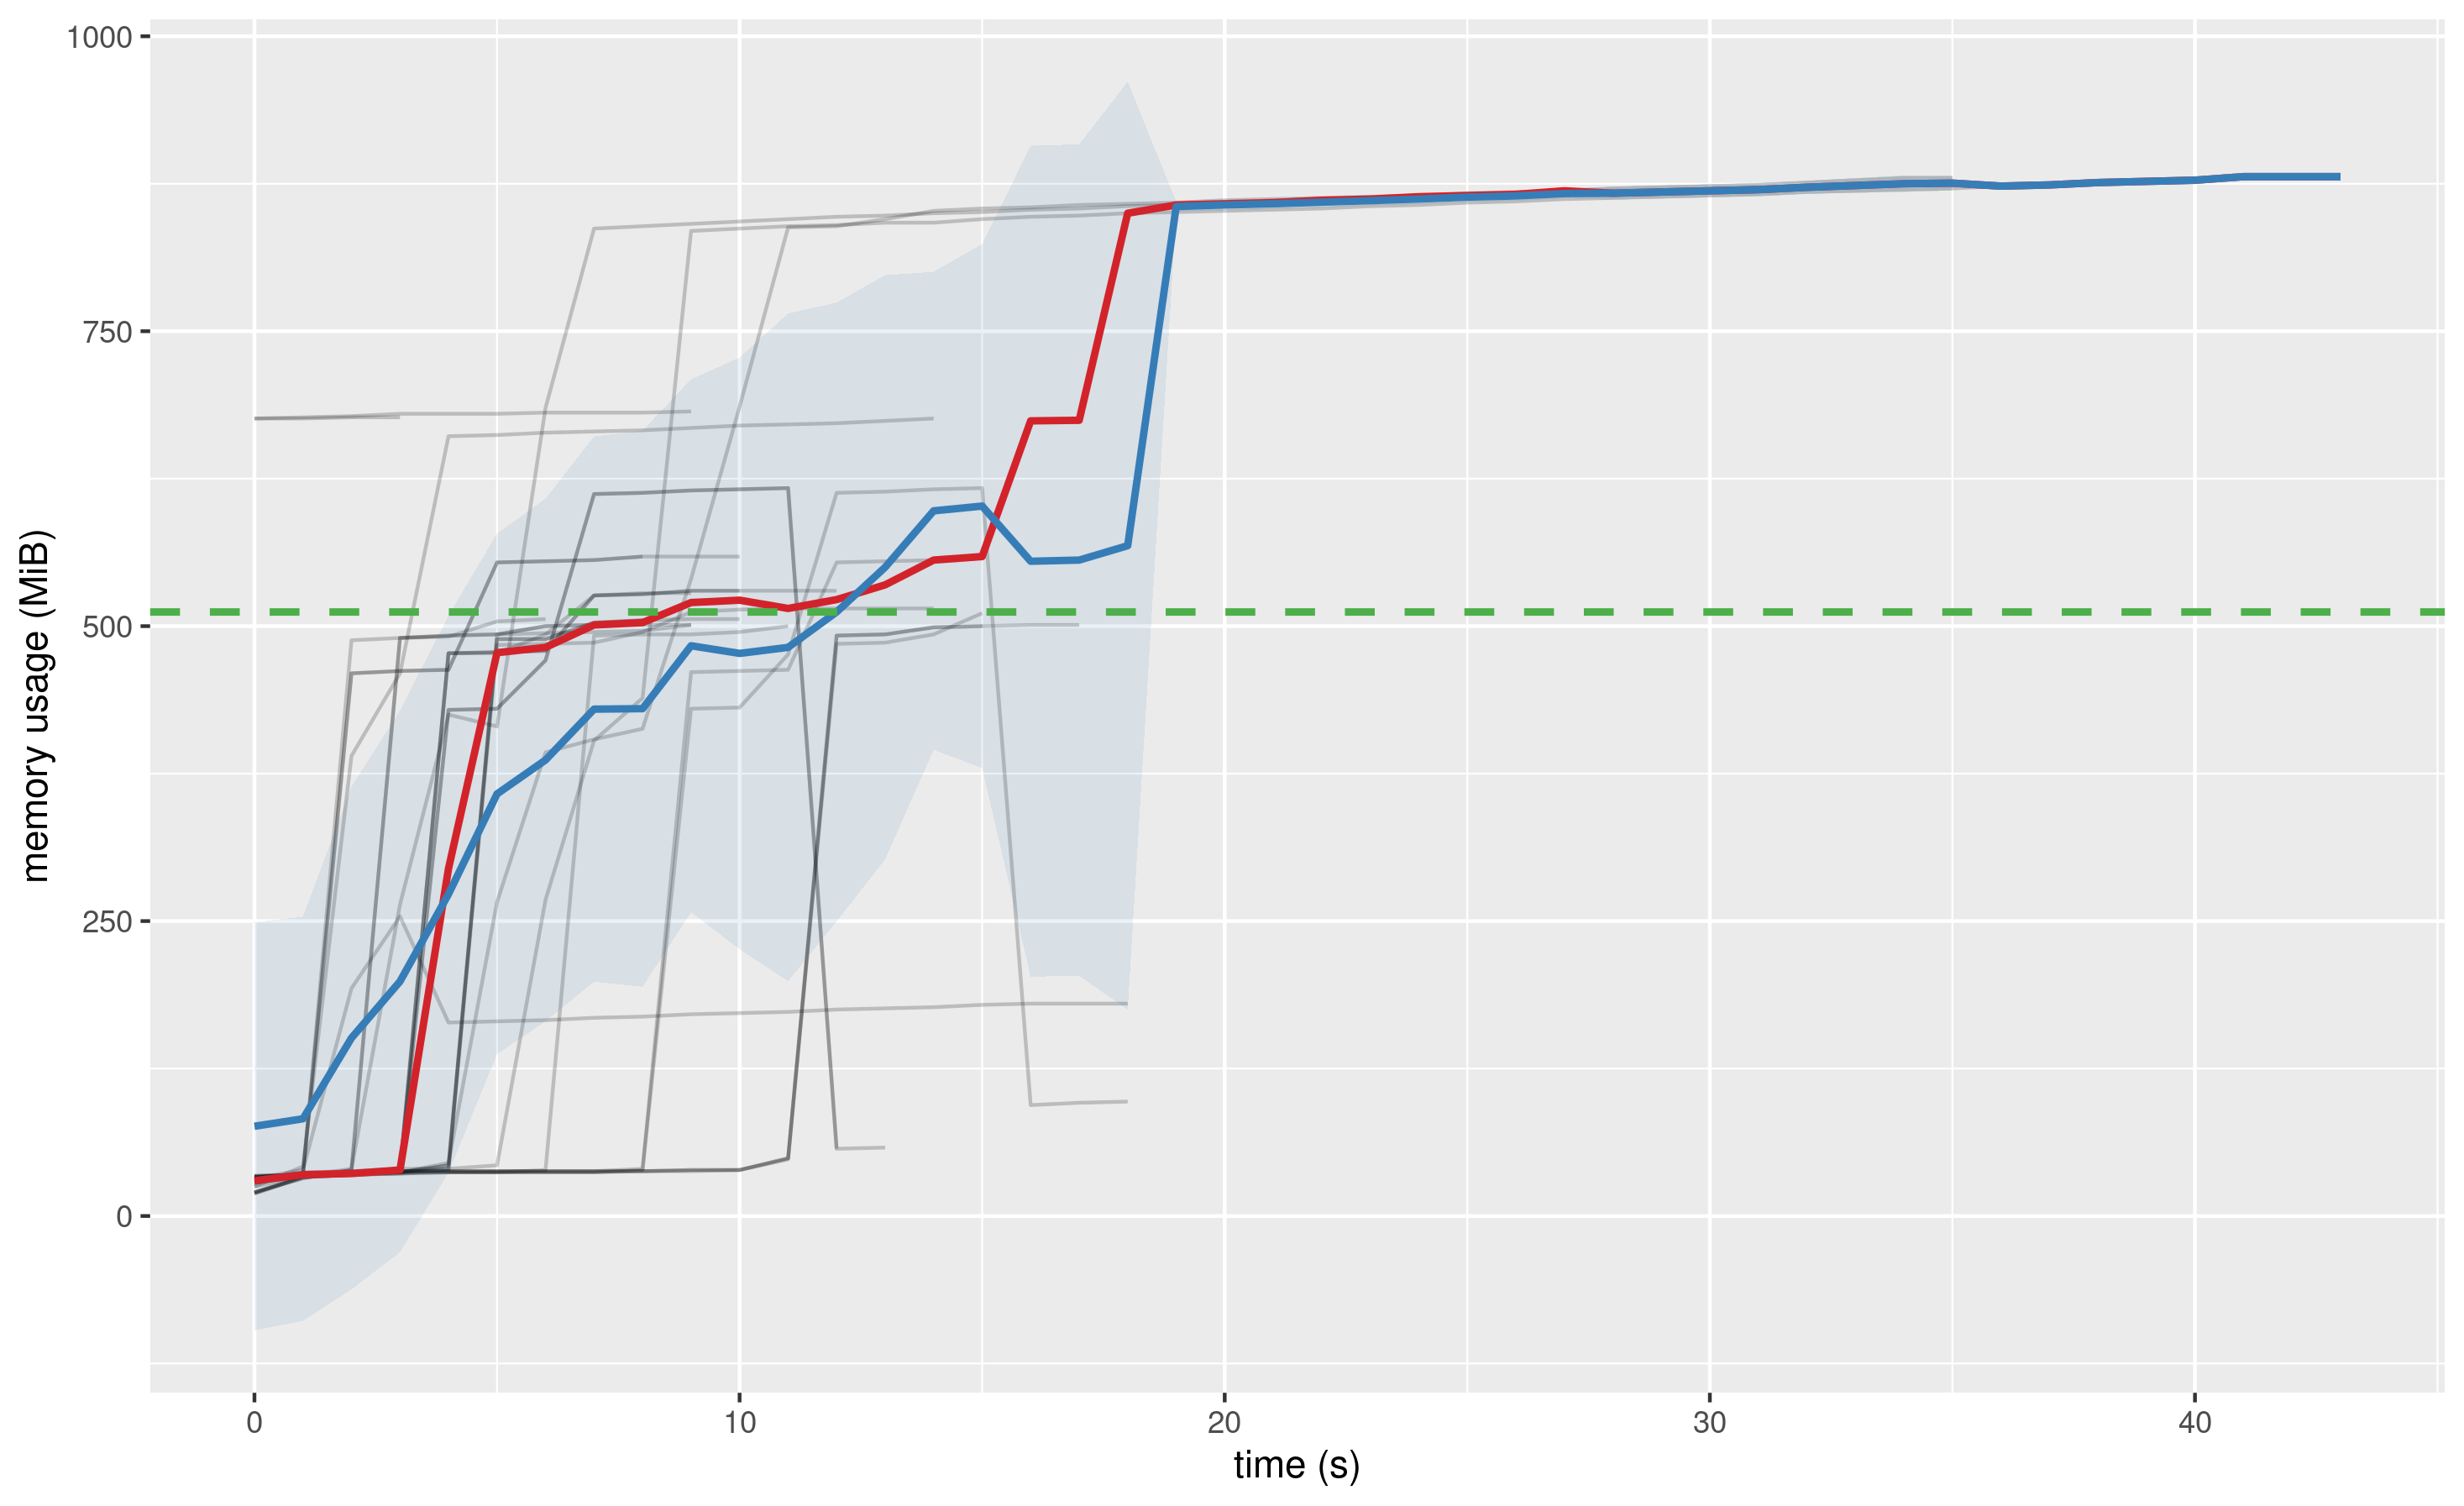
\includegraphics[width=\textwidth]{../plots/heap_512.png}
    \caption{expected heap usage: \SI{512}{\mebi\byte}}
    \label{fig:heap_512}
  \end{subfigure}
  \caption{Observed versus expected memory usage across time for four expected
    memory amounts. The green dashed horizontal line marks the expected amount
    of memory usage. Each gray line represents a different run. The red curve is
    their (pointwise) median, the blue curve is the mean, while the shaded area
    marks 1 standard deviation around the mean.}
  \label{fig:heap_experiment}
\end{figure}

\begin{figure}
  \centering
  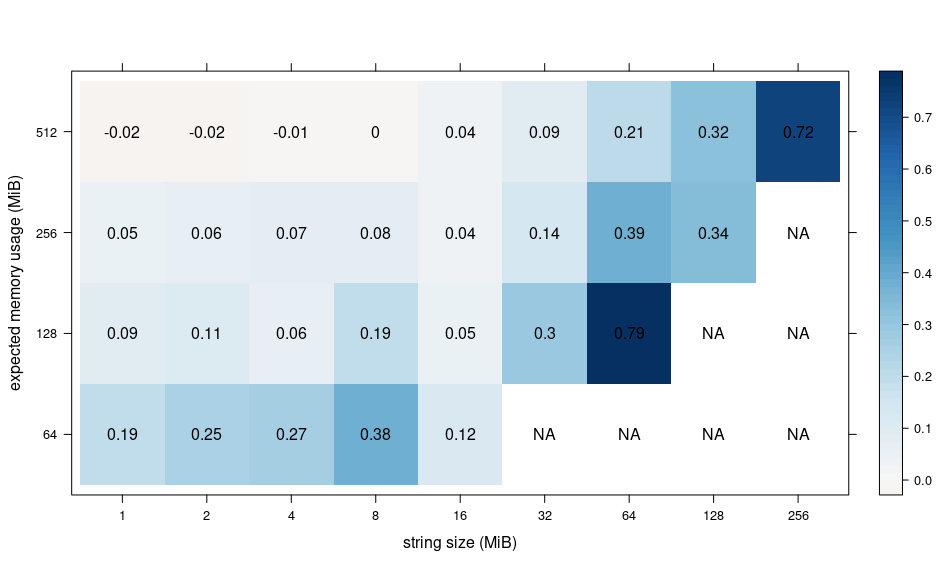
\includegraphics[width=\textwidth]{../plots/relative_median_errors.png}
  \caption{Relative median heap usage errors}
  \label{fig:relative_errors}
\end{figure}

\bibliographystyle{abbrv}
\bibliography{report}
\end{document}